\section{Fundamentos Teóricos}

\vspace{5 mm}

En este apartado explicaremos los principales fundamentos teóricos de las CNN's desde el punto de vista de Keras, que es la API que usaremos para desarrollar nuestro trabajo. Además, Keras es la API por excelencia para la construcción de CNN's.

\vspace{1 cm}

\subsection{¿Qué es una Red Neuronal Convolucional?}

\vspace{5 mm}

Una Red Neuronal Convolucional consiste en un conjunto de capas de filtros convolucionales de diferentes dimensiones. Estas capas son activadas por funciones de activación para dar no-linealidad a la red. Junto a estas capas se utilizan otras que aportan regularización, reducción de la dimensionalidad y aumento de la no-linealidad. El output de cada capa sirve como input de la capa a la que esté conectada. Un ejemplo de la estructura final de una CNN podría ser el siguiente:

\vspace{5 mm}

\begin{figure}[H]
  \centering
  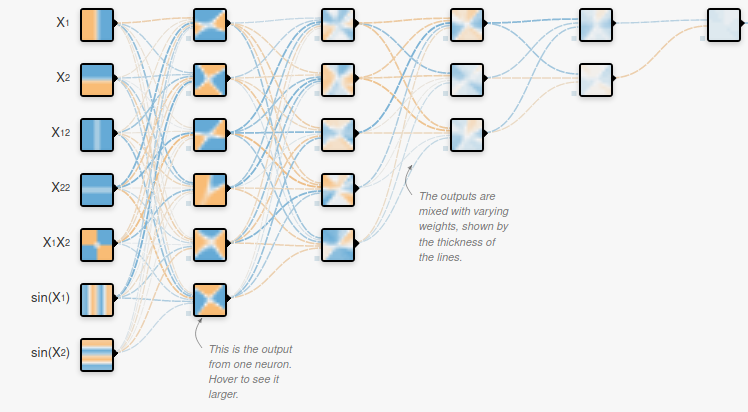
\includegraphics[width=0.5\linewidth]{Imagenes/cnn.png}
  \caption{CNN simulada en el Playground de TensorFlow}
  \label{fig:sub-first}
\end{figure}

\vspace{1 cm}

\subsection{Redes Neuronales Convolucionales para clasificación}

\vspace{5 mm}

Generalmente las Redes Neuronales Convolucionales para clasificación están formadas por capas \textbf{Conv2D}, \textbf{MaxPooling2D}, \textbf{Flatten} y \textbf{Dense}. También se usan activaciones \textbf{relu} y \textbf{softmax}. Estas capas serían las principales que toda arquitectura debería tener, pero hay muchas más.

\vspace{2 mm}

Las capas \textbf{Conv2D} producen tantas convoluciones 2D como \textbf{filters} indiquemos, usando un kernel de un tamaño \textbf{kernel\_size} que nosotros le damos. Los datos del kernel se corresponden con los pesos que ha aprendido la red neuronal hasta ese momento. La salida de una Conv2D es un bloque con tantos filtros convolucionados como indiquemos. Si no le indicamos ningún tipo de padding, las dimensiones de los filtros se verán reducidos a causa del kernel que se les pasa.

\vspace{2 mm}

Después de aplicar una capa convolucional o una capa Fully-Connected hay que aplicar una activación para modificar los valores de los filtros. Las activaciones se aplican porque en las últimas capas de nuestra red necesitamos extraer características de alto nivel que estén generalizadas para una clase particular.

\vspace{2 mm}

Por lo tanto, si no aplicasemos activaciones, los datos serían lineales y no podriamos alcanzar esa generalización que necesitamos en las últimas capas. Para darle no linealidad a los datos aplicamos dichas activaciones.

\vspace{2 mm}

En nuestro caso usaremos activaciones \textbf{relu}. Esta activación pasa los datos por la siguiente función:

\[g(z) = max(0, z)\]

De esta forma los datos negativos los convierte en 0, y los datos positivos los deja igual. Al aplicar esta función a los datos le estamos dando no linealidad a la red. Si representamos graficamente la activación obtenemos lo siguiente:

\vspace{5 mm}

\begin{figure}[H]
\centering
  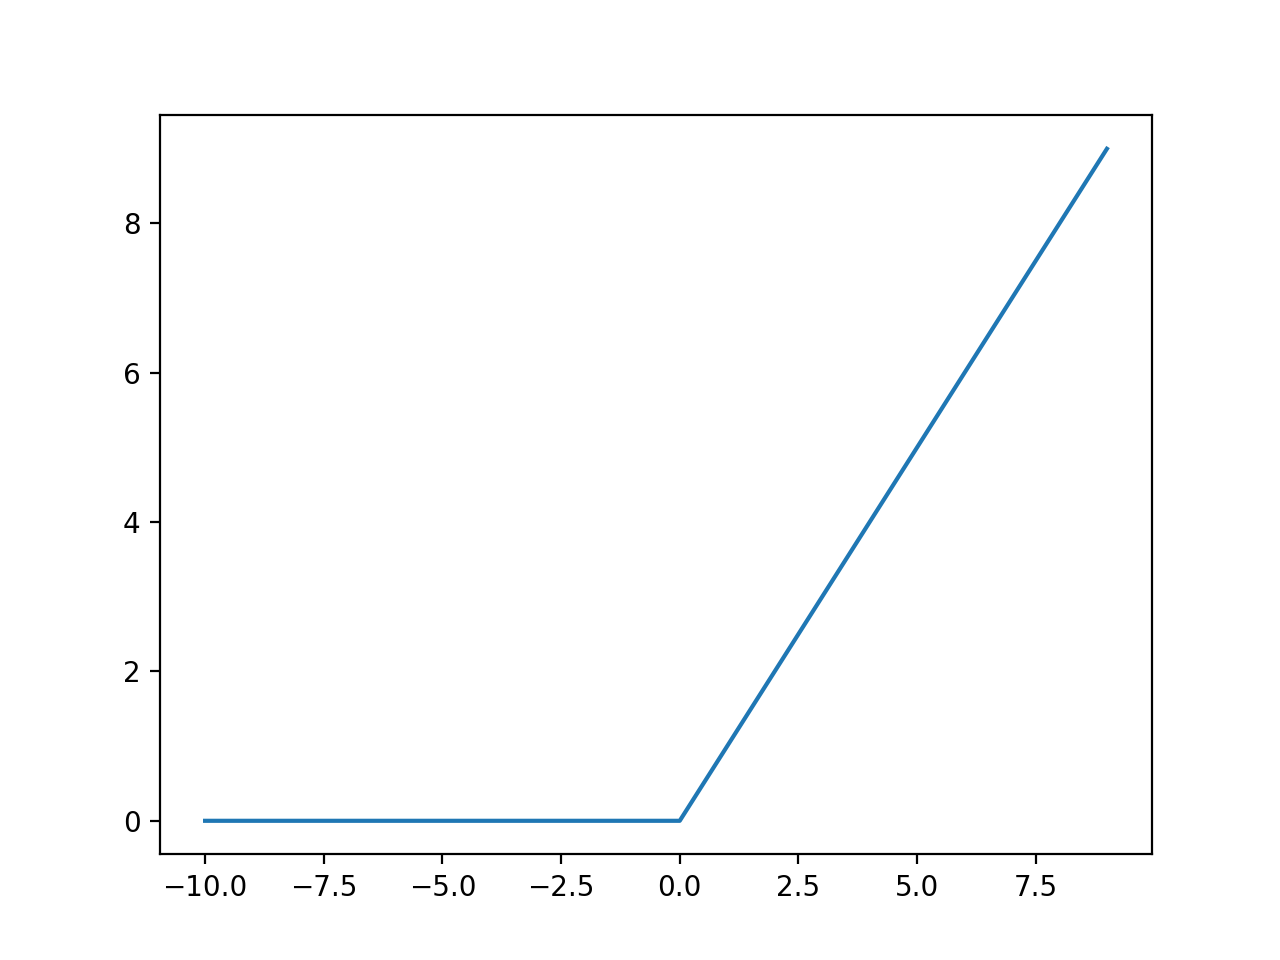
\includegraphics[width=0.5\textwidth]{Imagenes/relu.png}
   \caption{Activación Relu}
\end{figure}

\vspace{5 mm}

Vemos que los valores menores que 0 los toma directamente como 0.

\newpage

Las capas \textbf{MaxPooling2D} sirven para reducir la dimensionalidad de los filtros de tal manera que se reduce el coste computacional, también reduce la posibilidad de overfitting. Para ello utilizamos el hiperparámetro \textbf{pool\_size}. Lo que hace este valor es agrupar cada filtro en grupos de tamaño (pool\_size x pool\_size) y asignamos a cada grupo el valor máximo de los píxeles que forman el grupo. La idea se resume muy bien en la siguiente imagen:

\vspace{5 mm}

\begin{figure}[H]
\centering
  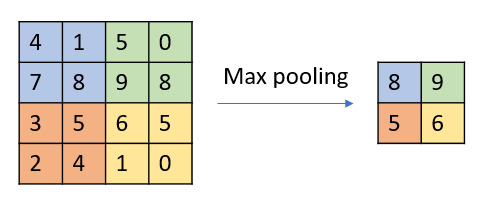
\includegraphics[width=0.5\textwidth]{Imagenes/pooling.jpg}
   \caption{MaxPooling2D de tamaño 2x2}
\end{figure}

\vspace{5 mm}

Las capas \textbf{Flatten} sirven para aplanar los bloques de filtros que tenemos hasta ese momento y convertirlos en un vector de n características. Para aplanar los filtros, lo que hace keras es multiplicar el \textbf{ancho} por el \textbf{alto} por el \textbf{numero de filtros} del que disponemos. Por ejemplo, si tuviesemos 6 filtros de 5x5, al aplicar Flatten() nos quedaríamos con un vector de 150 características.

\vspace{5 mm}

Las capas \textbf{Dense} son las conocidas como capas Fully-Connected, las cuales estan formadas por neuronas interconectadas entre si. La salida de la capa anterior se asigna a las neuronas de entrada de la capa fully-connected. A los datos que pasan por esta capa densa se les aplica una activación, en este caso \textbf{relu}, que aumenta la no linealidad del modelo. Normalmente hay menos neuronas en la salida de la capa densa que en la entrada.
La última capa de la red será otra fully-connected pero esta vez con activación \textbf{softmax}, de tal forma que tendrá tantas neuronas como clases tenga nuestra base de datos, y transformará los datos en la probabilidad de pertenecer a cada clase. La idea de las capas fully-connected se puede ver en la siguiente imagen:

\vspace{5 mm}

\begin{figure}[H]
\centering
  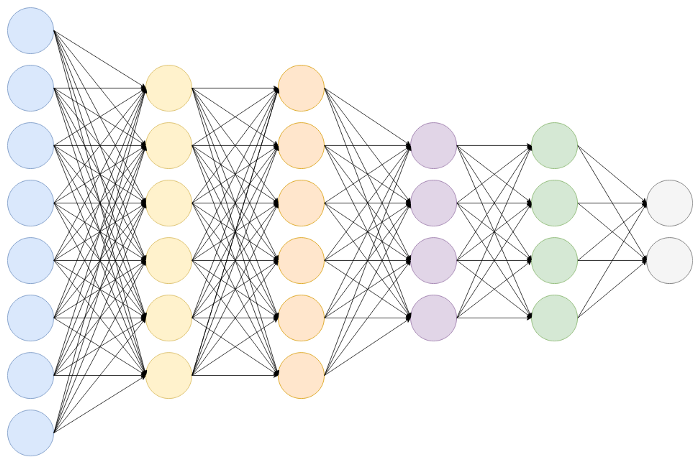
\includegraphics[width=0.5\textwidth]{Imagenes/fully.png}
   \caption{Capas Fully-Connected}
\end{figure}

\vspace{5 mm}

Una vez tenemos nuestro modelo, es necesario compilarlo usando una \textbf{función de pérdida}, un \textbf{optimizador} y una \textbf{métrica}.

\vspace{2 mm}

Como en este proyecto tenemos varias clases y cada imagen pertenece a una sola clase, vamos a usar como función de pérdida \textbf{categorical-crossentropy}. La entropía cruzada mide la distancia entre distribuciones de probabilidad y viene muy bien en nuestro caso porque la salida de nuestra red es un conjunto de probabilidades cuya suma es 1, ya que estamos usando una activación softmax en la última capa fully-connected.

\vspace{2 mm}

La función de pérdida es la siguiente:

\[Loss = - \sum_{i=1}^{output size}y_i * log (p_i) \]

Lo que hace esta función es, para cada conjunto de probabilidades de salida de nuestra red, ir sumando la multiplicacion de la etiqueta real de cada clase por la probabilidad que se ha calculado para esa clase. De tal forma que la única forma que tenemos de que la función de pérdida se quede en torno a cero, es multiplicar siempre la etiqueta correcta (1) por una probabilidad cercana a 1, ya que el logaritmo neperiano de 1 es 0. En nuestro caso estamos trabajando con una base de datos one-hot donde una sola etiqueta es correcta para cada imagen, por lo que el vector \textbf{"y"} estará lleno de 0 y solo tendrá un 1.

\vspace{2 mm}

Voy a ejemplificar esto con tres etiquetas para que se entienda mejor. Imaginemos que tenemos las etiquetas \textbf{perro}, \textbf{gato} y \textbf{pájaro} y que al introducir en nuestra red una imagen de un perro obtenemos las probabilidades \textbf{0.8}, \textbf{0.6} y \textbf{0.1} respectivamente. Nuestro vector \textbf{"y"} sería \textbf{[1,0,0]} en este caso porque la única etiqueta correcta es \textbf{perro}.

\vspace{2 mm}

Si aplicamos la función de pérdida explicada con estos datos obtenemos que:

\[Loss = - (1*log(0.8) + 0*log(0.6) + 0*log(0.1)) = 0.22\]


\vspace{2 mm}

Esta función se va a ir actualizando cada vez que pase una imagen por nuestra red y nuestro objetivo en todo caso va a ser minimizarla, ya que cuanto mas pequeña sea, mejor va a ser nuestro modelo. El encargado de minimizar esta función va a ser el \textbf{optimizador}.

\vspace{5 mm}

El \textbf{optimizador} utiliza la función de pérdida como guía para ir actualizando los pesos de la red. De tal forma que si la función de pérdida va disminuyendo, el optimizador sabe que los pesos que está usando van por el buen camino, y, si la función de pérdida aumenta, el optimizador sabe que tiene que cambiar los pesos.

\vspace{2 mm}

En este caso vamos a utilizar el optimizador \textbf{Adamax}, previamente estimado mediante GridSearchCV. Voy a intentar explicar lo que he entendido que hace con los pesos este optimizador. Antes de hablar de Adamax hay que hablar de \textbf{Adam}, ya que Adamax no es más que una generalización de Adam que va de la normalización \textbf{l2} a la normalización \textbf{l-infinity}. La normalización \textbf{l-infinity} es aquella que de un vector de valores, va a minimizar siempre el mayor de todos ellos.

\vspace{5 mm}

Sabemos que la función que utiliza Adam para ir actualizando los pesos es la siguiente:

\[w_t = w_{t-1} - lr  \frac{m_t}{\sqrt{v_t} + e} \]

Siendo lr el \textbf{learning rate}, y mt y vt estimadores del primer y segundo \textbf{momento} del gradiente respectivamente. La \textbf{e} es un valor muy pequeño que se utiliza para no dividir nunca entre 0.

\vspace{5 mm}

Pues sabiendo esto, lo que hace Adamax es una pequeña modificación de la función de actualización de pesos de Adam, quedándose así:

\[w_t = w_{t-1} - \frac{lr}{v_t} m_t   \]

Lo que nos dice la literatura es que Adamax es más robusto al ruido en los gradientes al usar esta nueva función de actualización de pesos. Se llega a ella mediante cálculos matemáticos que surgen de estar usando una normalización \textbf{l-infinity}.

\vspace{5 mm}

Finalmente nos va a hacer falta establecer una \textbf{métrica} a la hora de compilar nuestro modelo. La métrica no va a influir en el aprendizaje, si no que va a ser una manera de que podamos ver lo bien que esta prediciendo nuestro modelo en cada etapa. La métrica que vamos a usar en este caso es la \textbf{accuracy}. Esta métrica divide el número de clases bien predichas entre el total de clases. Por lo que si nuestro modelo predice bien 180 etiquetas de las 300 etiquetas totales, diremos que tiene una accuracy del 60 porciento.

\vspace{5 mm}

Anteriormente hemos estimado que el mejor inicializador de pesos posible para nuestro modelo es \textbf{he\_normal}. Este inicializador saca las muestras de una distribución normal truncada centrada en 0 y con la siguiente desviación típica:

\[stddev = sqrt(2 / fan_{in})\]

Donde fan\_in es el número de unidades de entrada en el tensor de pesos.
